\documentclass{beamer}
% Use UASLP1 theme if available, otherwise use Madrid
\IfFileExists{beamerthemeUASLP1.sty}{
    \usetheme{UASLP1}
}{
    \usetheme{Madrid}
    \usecolortheme{seahorse}
}

\usepackage[utf8]{inputenc}
\usepackage[T1]{fontenc}
\usepackage{helvet}
\usepackage{listings}
\usepackage{xcolor}
\usepackage{tikz}
\usepackage{hyperref}

% Code listing style
\lstset{
    basicstyle=\ttfamily\footnotesize,
    keywordstyle=\color{blue},
    commentstyle=\color{gray},
    stringstyle=\color{red},
    showstringspaces=false,
    breaklines=true,
    frame=single,
    numbers=left,
    numberstyle=\tiny\color{gray}
}

\title{Course 1: LoRa \& LoRaWAN}
\subtitle{Technical Deep Dive}
\author{Dr. ABDELMALEK OMAR}
\date{\today}
\institute{USP Zephyr Training Series\\Copyright \copyright{} 2025 Dr. ABDELMALEK OMAR}

\begin{document}

\begin{frame}[plain,t]
\titlepage
\end{frame}

\begin{frame}
\frametitle{Course Overview}
\framesubtitle{What You'll Learn}
\begin{itemize}
    \item LoRa Physical Layer
    \begin{itemize}
        \item Chirp Spread Spectrum modulation
        \item Link budget calculations
        \item Time-on-Air analysis
    \end{itemize}
    \item LoRaWAN Protocol
    \begin{itemize}
        \item MAC layer architecture
        \item Device classes (A, B, C)
        \item Join procedures (OTAA, ABP)
    \end{itemize}
    \item Hands-On Labs
    \begin{itemize}
        \item Lab 1.1: Link budget calculator
        \item Lab 1.2: Time-on-Air analysis
        \item Lab 1.3: OTAA join implementation
        \item Lab 1.4: Class C deployment
    \end{itemize}
\end{itemize}
\end{frame}

\section{LoRa Physical Layer}

\begin{frame}
\frametitle{What is LoRa?}
\framesubtitle{Long Range Radio Technology}

\begin{block}{Definition}
LoRa is a proprietary chirp spread spectrum (CSS) modulation technique developed by Semtech.
\end{block}

\begin{columns}[T]
\column{0.5\textwidth}
\textbf{Key Features:}
\begin{itemize}
    \item Long range (2-15 km)
    \item Low power (< 100 µA sleep)
    \item Low data rate (0.3-50 kbps)
    \item Robust to interference
\end{itemize}

\column{0.5\textwidth}
\textbf{Applications:}
\begin{itemize}
    \item Smart cities
    \item Agriculture sensors
    \item Asset tracking
    \item Utility metering
\end{itemize}
\end{columns}

\vspace{1em}
\begin{alertblock}{Proprietary Note}
LoRa PHY is proprietary (Semtech), but LoRaWAN MAC layer is open standard (LoRa Alliance).
\end{alertblock}
\end{frame}

\begin{frame}
\frametitle{Chirp Spread Spectrum}
\framesubtitle{How LoRa Modulates Data}

\begin{definition}[Chirp]
A chirp is a signal whose frequency increases (up-chirp) or decreases (down-chirp) linearly with time.
\end{definition}

\vspace{0.5em}

\begin{center}
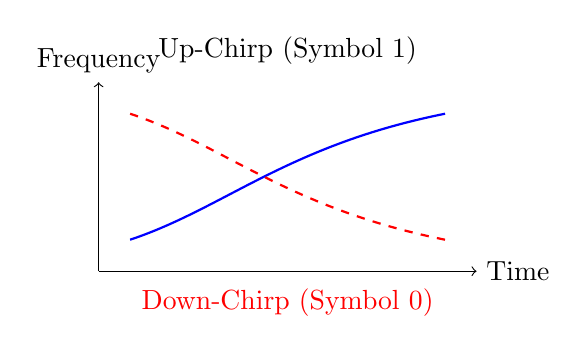
\begin{tikzpicture}[scale=0.8]
    % Axes
    \draw[->] (0,0) -- (6,0) node[right] {Time};
    \draw[->] (0,0) -- (0,3) node[above] {Frequency};

    % Up-chirp
    \draw[thick, blue] (0.5,0.5) .. controls (2,1) and (3,2) .. (5.5,2.5);
    \node at (3, 3.5) {Up-Chirp (Symbol 1)};

    % Down-chirp (dashed)
    \draw[thick, red, dashed] (0.5,2.5) .. controls (2,2) and (3,1) .. (5.5,0.5);
    \node at (3, -0.5) {\color{red} Down-Chirp (Symbol 0)};
\end{tikzpicture}
\end{center}

\begin{exampleblock}{Encoding Data}
Different data symbols are represented by chirps starting at different frequencies within the bandwidth.
\end{exampleblock}
\end{frame}

\begin{frame}
\frametitle{LoRa Parameters}
\framesubtitle{Configuration Options}

\begin{table}
\small
\begin{tabular}{|l|p{6cm}|}
\hline
\textbf{Parameter} & \textbf{Description} \\
\hline
Spreading Factor (SF) & 7-12. Higher SF = longer range, lower data rate \\
\hline
Bandwidth (BW) & 125, 250, 500 kHz. Wider BW = higher data rate \\
\hline
Coding Rate (CR) & 4/5, 4/6, 4/7, 4/8. More redundancy = more robust \\
\hline
TX Power & 2-20 dBm (EU), 2-30 dBm (US). Higher = longer range \\
\hline
Frequency & ISM bands: 868 MHz (EU), 915 MHz (US), 433 MHz (Asia) \\
\hline
\end{tabular}
\end{table}

\vspace{1em}

\begin{theorem}[Spreading Factor Trade-off]
Increasing SF by 1 doubles the range but halves the data rate and doubles Time-on-Air.
\end{theorem}
\end{frame}

\begin{frame}[fragile]
\frametitle{Link Budget Calculation}
\framesubtitle{Estimating Maximum Range}

\begin{block}{Link Budget Formula}
\[
RX_{power} = TX_{power} + TX_{gain} - PathLoss + RX_{gain} - Margin
\]
\end{block}

\textbf{Free Space Path Loss (FSPL):}
\[
FSPL(dB) = 20 \log_{10}(d_{km}) + 20 \log_{10}(f_{MHz}) + 32.45
\]

\begin{exampleblock}{Example Calculation}
\begin{itemize}
    \item TX Power: +14 dBm (EU868 limit)
    \item TX/RX Antenna Gain: 2 dBi each
    \item Frequency: 868 MHz
    \item Distance: 10 km
    \item LoRa Sensitivity (SF12): -137 dBm
\end{itemize}
\vspace{0.5em}
$FSPL = 20\log(10) + 20\log(868) + 32.45 = 131.4$ dB \\
$RX = 14 + 2 - 131.4 + 2 = -113.4$ dBm \\
$Margin = -113.4 - (-137) = 23.6$ dB {\color{green}\checkmark}
\end{exampleblock}
\end{frame}

\begin{frame}[fragile]
\frametitle{Time-on-Air (ToA)}
\framesubtitle{Airtime = Duty Cycle Compliance}

\begin{block}{Why ToA Matters}
EU868 regulation: Maximum 1\% duty cycle per sub-band per day (36 seconds/hour).
\end{block}

\textbf{ToA Formula (simplified):}
\[
ToA \approx \frac{2^{SF} \cdot PayloadBytes}{BW \cdot CR}
\]

\begin{table}
\footnotesize
\begin{tabular}{|c|c|c|c|}
\hline
\textbf{SF} & \textbf{ToA (10 bytes)} & \textbf{Max msgs/hour @ 1\%} \\
\hline
SF7  & 41 ms & 878 \\
SF8  & 72 ms & 500 \\
SF9  & 144 ms & 250 \\
SF10 & 247 ms & 145 \\
SF11 & 494 ms & 72 \\
SF12 & 991 ms & 36 \\
\hline
\end{tabular}
\end{table}

\begin{alertblock}{Duty Cycle Violation}
Exceeding 1\% duty cycle can result in regulatory fines and network bans!
\end{alertblock}
\end{frame}

\section{LoRaWAN Protocol}

\begin{frame}
\frametitle{LoRaWAN Architecture}
\framesubtitle{End-to-End Network}

\begin{center}
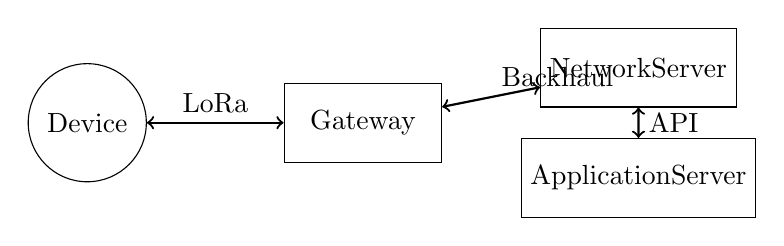
\begin{tikzpicture}[scale=0.7]
    % End Device
    \node[draw, circle, minimum size=1.5cm] (ed) at (0,0) {Device};

    % Gateway
    \node[draw, rectangle, minimum width=2cm, minimum height=1cm] (gw) at (5,0) {Gateway};

    % Network Server
    \node[draw, rectangle, minimum width=2cm, minimum height=1cm] (ns) at (10,1) {Network\\Server};

    % Application Server
    \node[draw, rectangle, minimum width=2cm, minimum height=1cm] (as) at (10,-1) {Application\\Server};

    % Connections
    \draw[<->, thick] (ed) -- (gw) node[midway, above] {LoRa};
    \draw[<->, thick] (gw) -- (ns) node[midway, above right] {Backhaul};
    \draw[<->, thick] (ns) -- (as) node[midway, right] {API};
\end{tikzpicture}
\end{center}

\begin{description}
    \item[End Device:] Battery-powered sensor transmitting data
    \item[Gateway:] Receives LoRa packets, forwards to network server via IP
    \item[Network Server:] Handles MAC layer, de-duplication, ADR
    \item[Application Server:] Your application logic, data storage
\end{description}
\end{frame}

\begin{frame}
\frametitle{Device Classes}
\framesubtitle{Class A, B, and C}

\begin{columns}[T]
\column{0.33\textwidth}
\textbf{Class A}
\begin{itemize}
    \item Lowest power
    \item TX + 2 RX windows
    \item Downlink only after uplink
    \item Latency: minutes
\end{itemize}

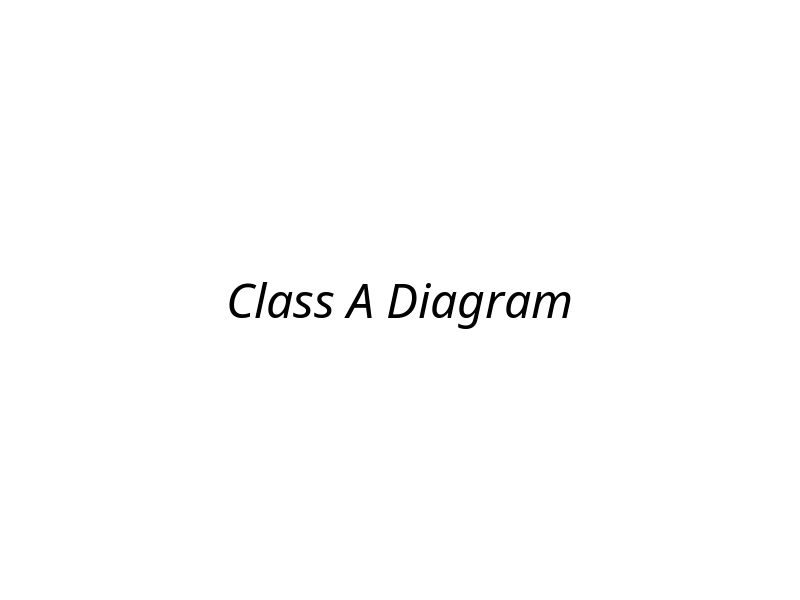
\includegraphics[width=\textwidth]{class_a_diagram.png}

\column{0.33\textwidth}
\textbf{Class B}
\begin{itemize}
    \item Scheduled RX slots
    \item Beacon synchronization
    \item Lower latency (seconds)
    \item Higher power
\end{itemize}

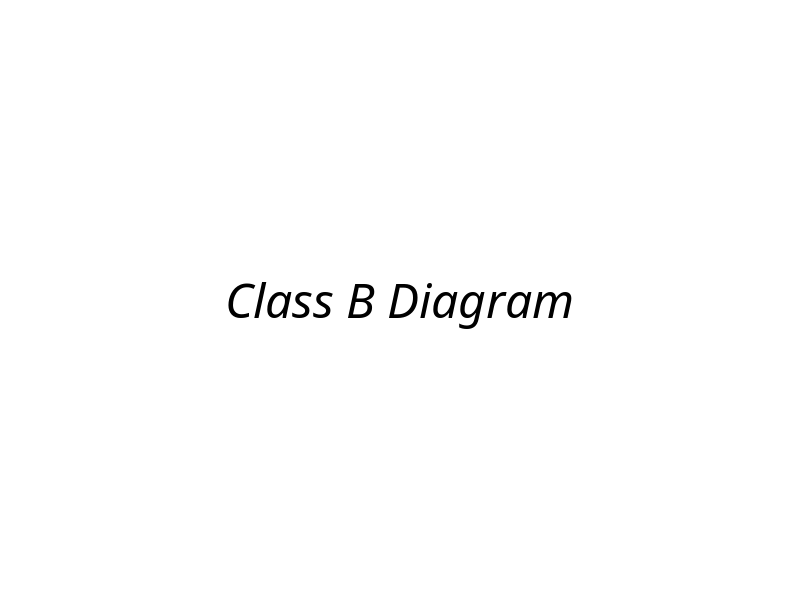
\includegraphics[width=\textwidth]{class_b_diagram.png}

\column{0.33\textwidth}
\textbf{Class C}
\begin{itemize}
    \item Continuous RX
    \item Lowest latency (instant)
    \item Highest power
    \item Mains-powered
\end{itemize}


\includegraphics[width=\textwidth]{class_c_diagram.png}
\end{columns}

\vspace{1em}

\begin{exampleblock}{Choosing a Class}
Class A = sensors | Class B = actuators | Class C = gateways/relays
\end{exampleblock}
\end{frame}

\begin{frame}[fragile]
\frametitle{OTAA vs ABP}
\framesubtitle{Device Activation Methods}

\begin{columns}[T]
\column{0.5\textwidth}
\textbf{OTAA (Recommended)}
\begin{itemize}
    \item Over-The-Air Activation
    \item Join procedure
    \item Dynamic session keys
    \item Secure
    \item Recovers from network reset
\end{itemize}

\vspace{1em}

\begin{lstlisting}[language=C, basicstyle=\tiny\ttfamily]
// OTAA credentials
uint8_t DevEUI[8] = {0x...};
uint8_t AppKey[16] = {0x...};

// Join network
smtc_modem_join_network(0);

// Wait for JOIN_ACCEPT
\end{lstlisting}

\column{0.5\textwidth}
\textbf{ABP (Legacy)}
\begin{itemize}
    \item Activation By Personalization
    \item Pre-provisioned keys
    \item Static session keys
    \item Less secure
    \item Frame counter issues
\end{itemize}

\vspace{1em}

\begin{lstlisting}[language=C, basicstyle=\tiny\ttfamily]
// ABP credentials
uint32_t DevAddr = 0x...;
uint8_t NwkSKey[16] = {0x...};
uint8_t AppSKey[16] = {0x...};

// No join needed
smtc_modem_set_app_skey(...);
smtc_modem_set_nwk_skey(...);
\end{lstlisting}
\end{columns}

\begin{alertblock}{Recommendation}
Always use OTAA for production deployments. ABP is for testing only.
\end{alertblock}
\end{frame}

\begin{frame}[fragile]
\frametitle{Adaptive Data Rate (ADR)}
\framesubtitle{Automatic Link Optimization}

\begin{block}{What is ADR?}
Network server instructs device to adjust spreading factor and TX power based on link quality.
\end{block}

\textbf{Benefits:}
\begin{itemize}
    \item Maximizes network capacity
    \item Minimizes power consumption
    \item Reduces collisions
\end{itemize}

\textbf{ADR Algorithm:}
\begin{enumerate}
    \item Device reports uplink with current DR and power
    \item Network server monitors RSSI/SNR over 20 uplinks
    \item If link margin > 15 dB, increase DR or reduce power
    \item If link margin < 5 dB, decrease DR or increase power
\end{enumerate}

\begin{exampleblock}{When to Disable ADR}
Disable ADR for mobile devices (vehicles, asset trackers) as link conditions change rapidly.
\end{exampleblock}
\end{frame}

\section{Hands-On Labs}

\begin{frame}[fragile]
\frametitle{Lab 1.1: Link Budget Calculator}
\framesubtitle{Python Implementation}

\textbf{Objective:} Calculate maximum range for different LoRa configurations.

\textbf{Deliverables:}
\begin{itemize}
    \item Python script implementing FSPL formula
    \item Test scenarios: SF7, SF10, SF12 at various distances
    \item Comparison table: Urban vs Rural vs Suburban
\end{itemize}

\vspace{1em}

\textbf{Example Output:}
\begin{verbatim}
Distance: 10 km, Frequency: 868 MHz
  SF7  (Sens: -123 dBm): Margin = 7.6 dB  [PASS]
  SF10 (Sens: -132 dBm): Margin = 16.6 dB [PASS]
  SF12 (Sens: -137 dBm): Margin = 21.6 dB [PASS]
\end{verbatim}

\vspace{1em}

\textbf{Learning Outcome:} Understand relationship between distance, SF, and link budget.
\end{frame}

\begin{frame}[fragile]
\frametitle{Lab 1.2: Time-on-Air Analysis}
\framesubtitle{Compliance Calculator}

\textbf{Objective:} Ensure duty cycle compliance for EU868.

\textbf{Tasks:}
\begin{enumerate}
    \item Calculate ToA for different payload sizes
    \item Determine maximum messages per hour (1\% duty cycle)
    \item Analyze impact of confirmed vs unconfirmed uplinks
\end{enumerate}

\vspace{1em}

\begin{lstlisting}[language=Python, basicstyle=\tiny\ttfamily]
def calculate_toa(sf, bw, payload_bytes, cr=1):
    """Calculate Time-on-Air in milliseconds"""
    symbol_time = (2**sf) / bw
    preamble_time = (8 + 4.25) * symbol_time

    payload_symbols = 8 + max(
        ceil((8*payload_bytes - 4*sf + 28) / (4*sf)) * (cr + 4),
        0
    )

    payload_time = payload_symbols * symbol_time
    return (preamble_time + payload_time) * 1000  # ms
\end{lstlisting}

\textbf{Learning Outcome:} Design compliant uplink schedules.
\end{frame}

\begin{frame}[fragile]
\frametitle{Lab 1.3: OTAA Join Implementation}
\framesubtitle{First LoRaWAN Application}

\textbf{Objective:} Join network and send periodic uplinks.

\textbf{Hardware:} Xiao-nRF54L15 + LR1120 shield

\vspace{1em}

\textbf{Code Skeleton:}
\begin{lstlisting}[language=C, basicstyle=\tiny\ttfamily]
int main(void) {
    // Initialize modem
    smtc_modem_init(event_handler);
    smtc_modem_set_region(STACK_ID, SMTC_MODEM_REGION_EU_868);

    // Start join
    smtc_modem_join_network(STACK_ID);

    while (1) {
        smtc_modem_run_engine();

        if (joined && time_for_uplink()) {
            uint8_t payload[] = {0x01, 0x02, 0x03};
            smtc_modem_request_uplink(STACK_ID, 2, false,
                                     payload, 3);
        }

        k_msleep(100);
    }
}
\end{lstlisting}

\textbf{Learning Outcome:} Understand LoRaWAN join flow and uplink scheduling.
\end{frame}

\begin{frame}
\frametitle{Lab 1.4: Class C Implementation}
\framesubtitle{Continuous Receive Mode}

\textbf{Objective:} Switch to Class C for immediate downlinks.

\textbf{Modifications:}
\begin{enumerate}
    \item After join, switch to Class C:
    \begin{itemize}
        \item \texttt{smtc_modem_set_class(STACK_ID, SMTC_MODEM_CLASS_C);}
    \end{itemize}
    \item Handle downlinks in \texttt{SMTC\_MODEM\_EVENT\_DOWNDATA}
    \item Measure power consumption difference
\end{enumerate}

\vspace{1em}

\textbf{Expected Results:}
\begin{table}
\footnotesize
\begin{tabular}{|l|c|c|}
\hline
\textbf{Metric} & \textbf{Class A} & \textbf{Class C} \\
\hline
Avg Current & 120 µA & 15 mA \\
Downlink Latency & ~60 seconds & < 1 second \\
Battery Life (2000 mAh) & 694 days & 5.6 days \\
\hline
\end{tabular}
\end{table}

\textbf{Learning Outcome:} Understand Class C trade-offs: latency vs power.
\end{frame}

\begin{frame}
\frametitle{Course 1 Summary}
\framesubtitle{Key Takeaways}

\textbf{You've Learned:}
\begin{itemize}
    \item LoRa PHY: CSS modulation, SF/BW/CR parameters
    \item Link Budget: Calculate max range using FSPL
    \item Time-on-Air: Ensure regulatory compliance
    \item LoRaWAN: MAC layer, device classes, OTAA
    \item Practical Skills: Build, flash, and test LoRaWAN devices
\end{itemize}

\vspace{1em}

\textbf{Next Steps:}
\begin{itemize}
    \item Course 2: LoRa Basics Modem Architecture
    \item Course 3: USP RAC for Multiprotocol
    \item Explore advanced features: FUOTA, Relay, Geolocation
\end{itemize}

\vspace{1em}

\begin{block}{Assessment}
Complete all 4 labs and pass the final quiz (80\%+) to earn Course 1 certificate.
\end{block}
\end{frame}

\begin{frame}[plain]
\centering
\Huge Thank You!

\vspace{2em}

\large Questions?

\vspace{2em}

\normalsize

\end{frame}

\end{document}
